\chapter{Propuesta}
\label{chap5}
\ifpdf
  \graphicspath{{Chapter5/Chapter5Figs/PNG/}{Chapter5/Chapter5Figs/PDF/}{Chapter5/Chapter5Figs/}}
\else
  \graphicspath{{Chapter5/Chapter5Figs/EPS/}{Chapter5/Chapter5Figs/}}
\fi

\markboth{\hfill \thechapter. Propuesta}{\hfill \thechapter. Propuesta}

\section{Planteamiento del problema}
\label{sec:planteamiento}

La fase de recolección de residuos sólidos cumple un rol importante en los aspectos socio-económicos y ambientales de una ciudad. Justamente, según la literatura, gran parte del presupuesto de un municipio va destinada a dicha fase. En consecuencia, se genera la necesidad de una búsqueda permanente por disminuir costos en sus procesos sin afectar la calidad del servicio. 

Hoy en día, la selección de la ruta de recolección se basa en la propia intuición y experiencia de los conductores. En la algunas ocasiones esto conlleva a dejar sin servicio algunos puntos de la ciudad por desconocimiento de un nuevo conductor asignado a la zona, que a su vez genera que la comuna asuncena realice quejas acerca de la falta de servicio de recolección en tiempo y forma. También es posible el paso en repetidas veces de forma innecesaria por la misma calle dando lugar a mayores gastos de combustible, como se observa indicado en los círculos rojos de la ``Fig.~\ref{fig:trayectoRecoleccion}''.

Otra situación muy común es el continuo cambio de circulación en las calles con el fin de disminuir la congestión del tráfico actual, como por ejemplo: cambio de sentido, prohibición de giro a la izquierda, giro en U, contramano. Muchas veces la calles quedan clausuradas para su uso por motivo de reparación de la capa asfáltica, trabajos de instalación o reparación de cañería. 

Para ello se implementa una solución GIS que optimice el camino del vehículo recolector teniendo en cuenta el procedimiento actual llevado a cabo para la recolección de residuos domiciliarios, gestionando de forma sencilla y rápida el estado actual de las calles y sus reglas de circulación. A continuación se detalla la solución propuesta.

\begin{figure}[H]
    \centering
    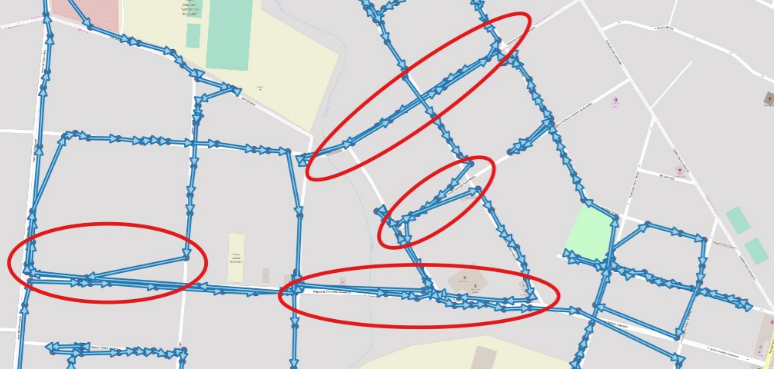
\includegraphics[width=14.5cm]{20170329_recorrido_repetido.png}
    \caption{Trayecto del vehículo 62 en fecha 11 de Julio del 2016 en el turno mañana. [Fuente: Datos de rastreo vía GPS desplegados en la aplicación QGis]}
    \label{fig:trayectoRecoleccion}
\end{figure}

Los siguientes supuestos son establecidos para la solución planteada:

\begin{itemize}
    \item El vehículo recolector cuenta con capacidad suficiente para recoger los residuos de una zona determinada.
    \item El tráfico es constante en una zona de trabajo en el turno en que se recogen sus residuos.
    \item Las modificaciones geográficas de los datos espaciales estarán a cargo de una persona capacidad en el área GIS.
    % La persona encargada de la administración del sistema posee conocimientos básicos en GIS y podrá actualizar, crear y eliminar una zona de trabajo mediante el sistema \textit{QGis}
\end{itemize}


% En la Figura \ref{fig:trayectoRecoleccion}, se muestra una pequeña parte del rastreo de una zona, en los círculos de color rojo se pueden observar como el mismo vehículo recorre la misma calle más de una vez. Esta situación se pudo contemplar en los recorridos de varias zonas. Para la recolección de datos se solicitó a la DSU el permiso de instalar un dispositivo GPS a un vehículo recolector de basura, como parte de este proyecto, a través del cual obtuvimos por un periodo de 3 meses los datos de posicionamiento relacionados al vehículo 62 de propiedad de la Municipalidad de Asunción. Esta idea ya generó el interés de la Municipalidad de Asunción, que posteriormente ha realizado una licitación para dotar a todos los vehículos recolectores de residuos un dispositivo similar GPS, brindándonos acceso a los datos del rastreo de todos vehículos recolectores.

\section{Solución planteada}

En la ``Fig.~\ref{fig:metodologia}'' se muestra la metodología seguida en este trabajo: la recolección de datos, el modelado matemático, la implementación de la herramienta \textit{TapeYty}, el despliegue de la ruta óptima y por último el análisis de los resultados.

\begin{figure}[tbp]
\centerline{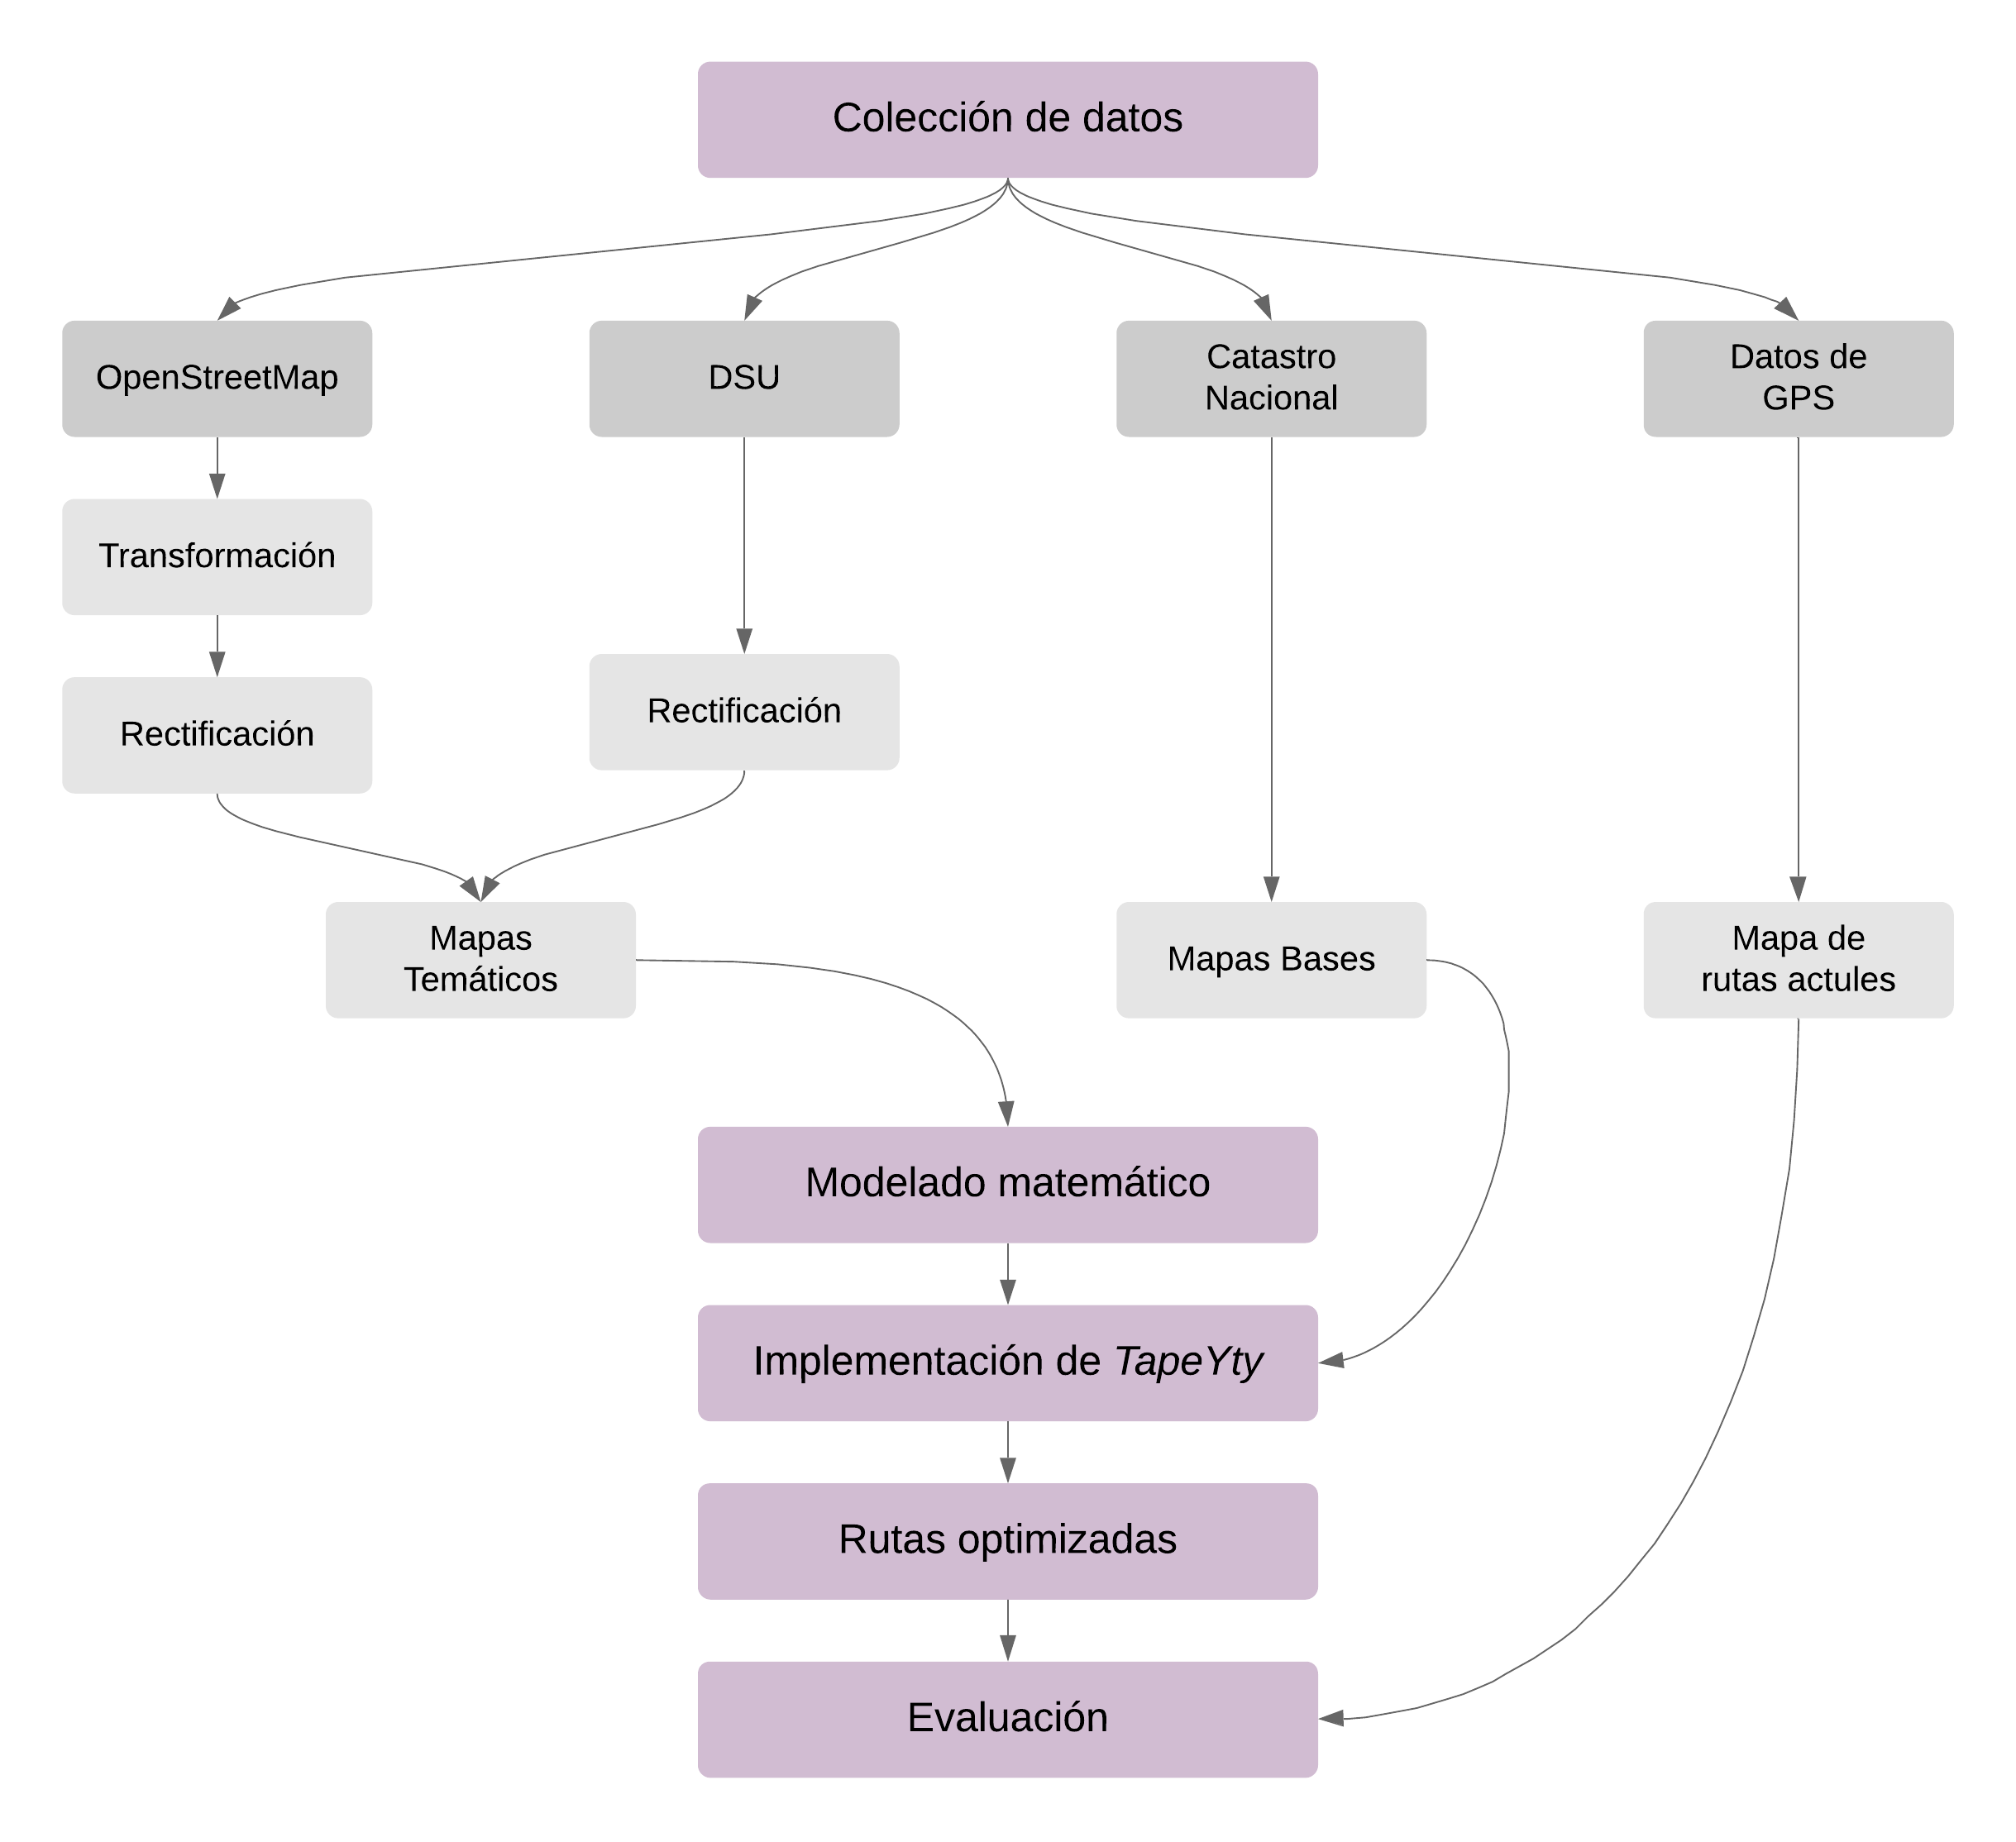
\includegraphics[width=9.5cm]{DiagramaDeMetodologia.png}}
\caption{Procedimientos de la metodología.}
\label{fig:metodologia}
\end{figure}

% La solución del trabajo de investigación es lo que se buscará encontrar en el transcurso del desarrollo del TFG. La solución encontrada debe permitir obtener mejores resultados en cuanto a costo de recolección, en comparación a la situación actual en la DSU del municipio de Asunción, así como también, generar resultados óptimos que contribuyan con el estado del arte actual

\subsection{Colección de Datos}

Se crea una base de datos espacial utilizando el gestor de base de datos de código abierto PostgreSQL, junto con su extensión PostGIS que brinda soporte de objetos geográficos.

Se necesitó exportar los datos de Asunción desde OSM, debido a que no se tuvo conocimiento de alguna institución que proveyera de mapas de calles de la ciudad con sus sentidos. A continuación se detallan los pasos seguidos para obtener la red de rutas utilizada: 
\begin{itemize}
\item Se utiliza la herramienta \textit{osm2pgsql} para importar los datos de OSM a la base de datos, en el sistema de referencia geográfico WGS84 (SRID 4326). 
\item Se utiliza las funciones de PostGIS para convertir los valores de latitud y longitud al tipo de dato geométrico \textit{Point}, es decir, un Punto. 
\item Las calles de OSM están representadas por líneas, que a su vez contienen una serie de nodos (puntos). Se excluyen los puntos que no pertenecen a calles de la ciudad, además de puntos superpuestos. 
\item Para un mejor manejo de la red de rutas se crea un proceso de segmentación de las calles, donde cada segmento de calle está formado por pares de nodos consecutivos, se define el sentido del segmento, longitud y si el segmento de calle es un callejón sin salida. 
\item Se realizan las transformaciones correspondientes para almacenar las restricciones de giro y contramano.
\end{itemize}

La delimitación de las zonas de recolección fue proveída por la DSU a través de un archivo \textit{shape} del tipo de dato geométrico \textit{Polygon}, es decir, un Polígono:
\begin{itemize}
\item Se importa a la base de datos mediante la herramienta \textit{shp2pgsql}.
\item Se usa la aplicación QGIS para la limpieza y corrección de datos geográficos, haciendo coincidir los límites de las zonas de recolección con las calles de OSM.
\end{itemize}

El Sistema Nacional de Catastro provee los mapas bases de Departamentos y Distritos a la aplicación a través de su portal de datos abiertos. 

La DSU cuenta en algunos vehículos de su flota con un sistema de monitoreo mediante el Sistema de Posicionamiento Global (GPS, \textit{Global Positioning System}). 

\begin{itemize}
    \item Se accede a los datos a través de archivos en formato Microsoft Excel para su posterior importación a la base de datos. 
    \item Esta información será utilizada para el análisis y comparación de los resultados.
    %  \item Se aplica el método map matching esta información será utilizada para el análisis y comparación de los resultados.
\end{itemize}

\subsection{Modelo matemático}

Como resultado de la revisión del estado del arte, se utiliza la solución propuesta por \citet{Braier2017AnArgentina} para optimizar el enrutamiento de vehículos recolectores. Este modelo se selecciona debido a las similitudes con el caso de estudio de este trabajo, entre ellas es posible citar:

\begin{itemize}
    \item División de la ciudad en sectores y recolección casa por casa: La situación es muy similar, ya que el procedimiento consiste en recoger los residuos domiciliarios casa por casa, debiendo cubrir todas las calles de un conjunto de cuadras o manzanas, denominadas zonas.
    \item Tamaño de problema: Una zona de recolección abarca en promedio el mismo número (entre 40 y 80 cuadras aproximadamente), que representa un número aceptable para la solución utilizada.
    \item Calles, carreteras, caminos: el trabajo de \citet{Braier2017AnArgentina} tomó como caso de estudio la ciudad de Morón el cuál presenta caminos con particularidades muy comunes a otras sudamericanas como la de Asunción: calles sin salida, calles estrechas, peatonales, giros prohibidos, entre otros.
\end{itemize}

Además, la falta de datos relacionados con la cantidad de toneladas recolectadas por zonas fue otro de los principales motivos por el cual se seleccionó un problema de ruta cuya demanda se encuentra sobre los arcos (calles que deben ser visitadas), y además no posea restricciones de capacidad.

Cada zona de recolección de la ciudad de Asunción es representada por un grafo mixto $H$ \citep{Braier2017AnArgentina}, cuyos nodos representan las esquinas de las calles en la zona, y los arcos son los segmentos de calles que corren entre dos intersecciones consecutivas. Las calles de un único sentido están representadas por arcos dirigidos y las calles finas de doble sentido por arcos no dirigidos, ya que ambos lados de la calle pueden ser servidos en un solo viaje. En el caso de calles anchas de doble sentido, como las avenidas, cada lado debe ser servido de forma separada, por lo que estas calles se representan con dos arcos dirigidos, una en cada sentido.

Para incorporar las restricciones de regulación de tráfico se construye un grafo dirigido $G$ desde el grafo $H$. El grafo $H$ es expandido dividiendo cada nodo en varios nuevos nodos representando todas las formas en las que se puede llegar y salir de la esquina en cuestión. En la ``Fig.~\ref{fig:grafo_expandido}(a)'' se puede observar un nodo en el grafo original $H$ antes de su expansión, y en la ``Fig.~\ref{fig:grafo_expandido}(b)'' el nodo que ha sido expandido en seis nuevos nodos, representando cada posible entrada y salida del nodo. Los arcos auxiliares dirigidos son agregados y conectan los nuevos nodos, representando así las transiciones permitidas de una esquina a otra.

El modelo de programación entera propuesto por \citet{Braier2017AnArgentina} está definido de la siguiente manera:

\subsubsection{Conjuntos y Parámetros}
\label{sec:conjunto-parametros}

\begin{itemize}
\item $G(V, A)$: Grafo dirigido en el que los nodos V corresponden a todas las alternativas posibles para llegar a las esquinas de las intersecciones y A está compuesto por arcos que se pueden atravesar en una sola dirección específica.

\item $E \subseteq \{ \{i, j\}: i \in V, j \in V, i \neq j\}$: Representan segmentos de calles de dos vías que pueden ser recorridos en cualquier sentido.

\item $AM \subseteq A $: Arcos obligatorios que representan segmentos que deben recorrerse únicamente en el sentido especificado.

\item $w : A \rightarrow \mathbb{R} $: Función de peso que asocia un peso a cada arco, en este caso la distancia del segmento de calle. Los arcos auxiliares entre nodos que representan esquinas tienen un mismo valor ínfimo.

\item $I \subseteq V $: Nodos que especifican los puntos de inicio permitidos para la ruta.

\item $S \subseteq V$: Se define $\delta^+ (S) = \{i j \in A: i \in S , j \notin S \}$ , que representa un conjunto de arcos que van desde nodos en $S$ a nodos en $V \backslash S$.
\end{itemize}

El problema de ruteo es una versión particular del problema del cartero rural abierto dirigido, ya que el arco $i j \in E $ determina el grupo de arcos $L_{i j} = \{i j, j i\}$, en el que al menos uno de ellos debe ser atravesado en la solución final y además se busca un camino cuyo nodo inicial y final no se especifican.

\begin{figure}[tbp]
\centerline{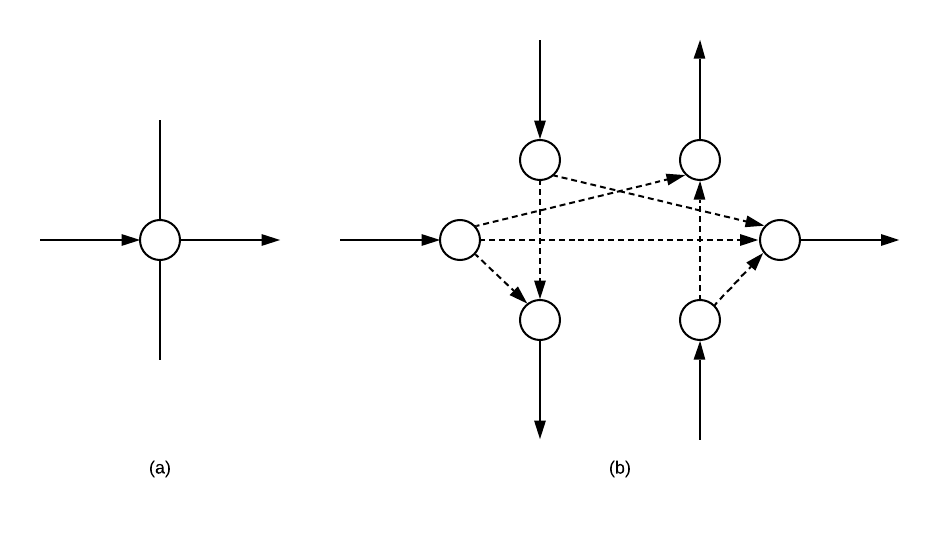
\includegraphics[width=9.5cm]{expanded_graph.png}}
\caption{Expansión de un cruce entre una calle de sentido único y una calle de doble sentido. (a) Grafo mixto original. (b) Grafo dirigido luego de la expansión, los arcos auxiliares están representados por líneas discontinuas. [Fuente: \citet{Braier2017AnArgentina}]}
\label{fig:grafo_expandido}
\end{figure}

\subsubsection{Variables de decisión}
\begin{itemize}
\item $x_{i j}$: Para cada arco $ {i j} \in A$ esta variable representa el número de veces que $i j$ es atravesado.

\item $s_i$: Para cada nodo $i \in I$ esta variable binaria especifica si  $i$ es el primer nodo de la ruta.

\item $t_j$: Para cada nodo $j \in V$ esta variable binaria indica si $j$ es el último nodo de la ruta.
\end{itemize}

\subsubsection{Definición del programa entero}
\label{sec:programa-entero}
\begin{equation*}
\min \sum_{i j \in A} w_{i j} x_{i j}  \\
\end{equation*} 
\hbox{}

\begin{equation} \tag{1} \label{eq1}
\begin{gathered}
x_{i j} \geq 1 \\
\forall i j \in A M
\end{gathered}
\end{equation} 
\hbox{}

\begin{equation} \tag{2} \label{eq2}
\begin{gathered}
x_{i j} + x_{j i} \geq 1 \\
\forall i j \in E
\end{gathered}
\end{equation}
\hbox{}

%ecuacion 3a
\begin{equation} \tag{3a} \label{eq3a}
\begin{gathered}
s_i + \sum_{j: j i \in A} x_{j i} = \sum_{j: i j \in A} x_{i j} + t_i \\
\forall i \in I
\end{gathered}
\end{equation} 
\hbox{}

%ecuacion 3b
\begin{equation} \tag{3b} \label{eq3b}
\begin{gathered}
\sum_{j: j i \in A} x_{j i} = \sum_{j: i j \in A} x_{i j} + t_i \\
\forall i \in V\backslash I
\end{gathered}
\end{equation}
\hbox{}

\begin{equation} \tag{4} \label{eq4}
\sum_{i \in I} s_i = 1 
\end{equation}
\hbox{}

\begin{equation} \tag{5} \label{eq5}
\sum_{i \in V} t_i = 1 
\end{equation}
\hbox{}

\begin{equation} \tag{6} \label{eq6}
\begin{gathered}
    \sum_{i j \in \delta + (S)} x_{i j} \geq 1 \\
    \forall S \subseteq V
\end{gathered}
\end{equation}
\hbox{}

\begin{equation} \tag{7} \label{eq7}
\begin{gathered}
    x_{i j} \in \mathbb{Z}_+ \\
    \forall i j \in A
\end{gathered}
\end{equation}
\hbox{}

\begin{equation} \tag{8} \label{eq8}
\begin{gathered}
    s_i \in \{0,1\} \\
    \forall i \in I
\end{gathered}
\end{equation}
\hbox{}

\begin{equation} \tag{9} \label{eq9}
\begin{gathered}
    t_i \in \{0,1\} \\
    \forall i \in V
\end{gathered}
\end{equation}

La función objetivo busca minimizar el costo total de la ruta de recolección de residuos. El costo total se refiere a la distancia recorrida por el vehículo recolector. La restricción (\ref{eq1}) impone que todos los arcos de único sentido deben ser visitados al menos una vez, la (\ref{eq2}) requiere que los arcos no dirigidos sean atravesados al menos una vez en cualquier sentido. Las restricciones (\ref{eq3a}) y (\ref{eq3b}) aseguran que la solución encontrada es realmente un camino agregando la condición de conservación de flujo estándar a cada nodo. Las restricciones (\ref{eq4}) y (\ref{eq5}) garantizan que el nodo inicial y final sean únicos. Las restricciones (\ref{eq1})-(\ref{eq5}) permiten la formación de subtours, la restricción (\ref{eq6}) es el estándar de eliminación de subtours. Las restricciones (\ref{eq7})-(\ref{eq9}) especifican los valores posibles para las variables del modelo.

\subsubsection{Algoritmo de solución}
\label{algoritmo-solucion}
% En el modelo dado en la sección \ref{sec:programa-entero} se puede observar la restricción de eliminación de subtours la cual es muy costosa en la generación de las mismas como también en  la complejidad del problema. En este contexto la estrategia propuesta en \cite{Braier2017AnArgentina} se basa en tratar de obtener una solución rápidamente sin considerar el problema de subtour e ir agregando las restricciones sucesivamente, esto se conoce como técnica de agregación dinámica de restricciones a un modelo relajado.

En el modelo dado en la sección \ref{sec:programa-entero} se puede observar la restricción de eliminación de subtours la cual es muy costosa en la generación de las mismas como también en la complejidad del problema. En este contexto la estrategia propuesta en \citet{Braier2017AnArgentina} se basa en tratar de obtener una solución rápidamente sin considerar el problema de subtour, en caso de que existan subtours se eliminan mediante el procedimientos de mezcla de subtours, si no se puede utilizar esta técnica se van agregando las restricciones sucesivamente, esto se conoce como técnica de agregación dinámica de restricciones a un modelo relajado.

Los siguientes pasos detallan la estrategia:

\begin{enumerate}
\item Crear el modelo relajado $M: = (\ref{eq1}) - (\ref{eq5})$ y $(\ref{eq7}) - (\ref{eq9})$.
\item Resolver $M$.
\item Si no se puede encontrar ninguna solución para $M$, retornar ``infactible'' y parar.
\item Si la mejor solución encontrada para $M$ no tiene subtours, retornar esta solución y parar.
\item Si los subtours pueden ser mezclados con el tour que contiene el nodo inicial y final, entonces mezclarlos, retornar la solución obtenida y parar.
\item De lo contrario, agregar a $M$ la restricción de eliminación de subtour estándar (\ref{eq6}) por cada subtour en la solución y regresar al paso 2.
\end{enumerate}

El procedimiento de mezcla de subtours descrito por \citet{Braier2017AnArgentina}, utilizado en el paso 5, consiste en que dado un subtour \textit{S} y el camino principal \textit{P}, es decir el camino que empieza en el único vértice $i \in I$ con $s_i = 1$, y termina respectivamente en $t_i = 1$, se intenta intercambiar los arcos auxiliares para mezclar \textit{S} y \textit{P}. Se puede presentar una de las siguientes tres configuraciones:

\begin{itemize}
    \item Configuración A: Si el camino principal y el subtour se encuentran en algún nodo intermedio, como en la ``Fig.~\ref{fig:procedimiento_mezcla_subtours}(a)'', entonces son unidos como en la ``Fig.~\ref{fig:procedimiento_mezcla_subtours}(b)''
    \item Configuración B: Si el subtour se encuentra con el último nodo en la ruta principal, como en la ``Fig.~\ref{fig:procedimiento_mezcla_subtours}(c)'', entonces se unen como en la ``Fig.~\ref{fig:procedimiento_mezcla_subtours}(d)''.
    \item Configuración C: Si el subtour se encuentra con el primer nodo en la ruta principal, como en la ``Fig.~\ref{fig:procedimiento_mezcla_subtours}(e)'', entonces se unen como en la ``Fig.~\ref{fig:procedimiento_mezcla_subtours}(f)''.
\end{itemize}

\begin{figure}[tbp]
\centerline{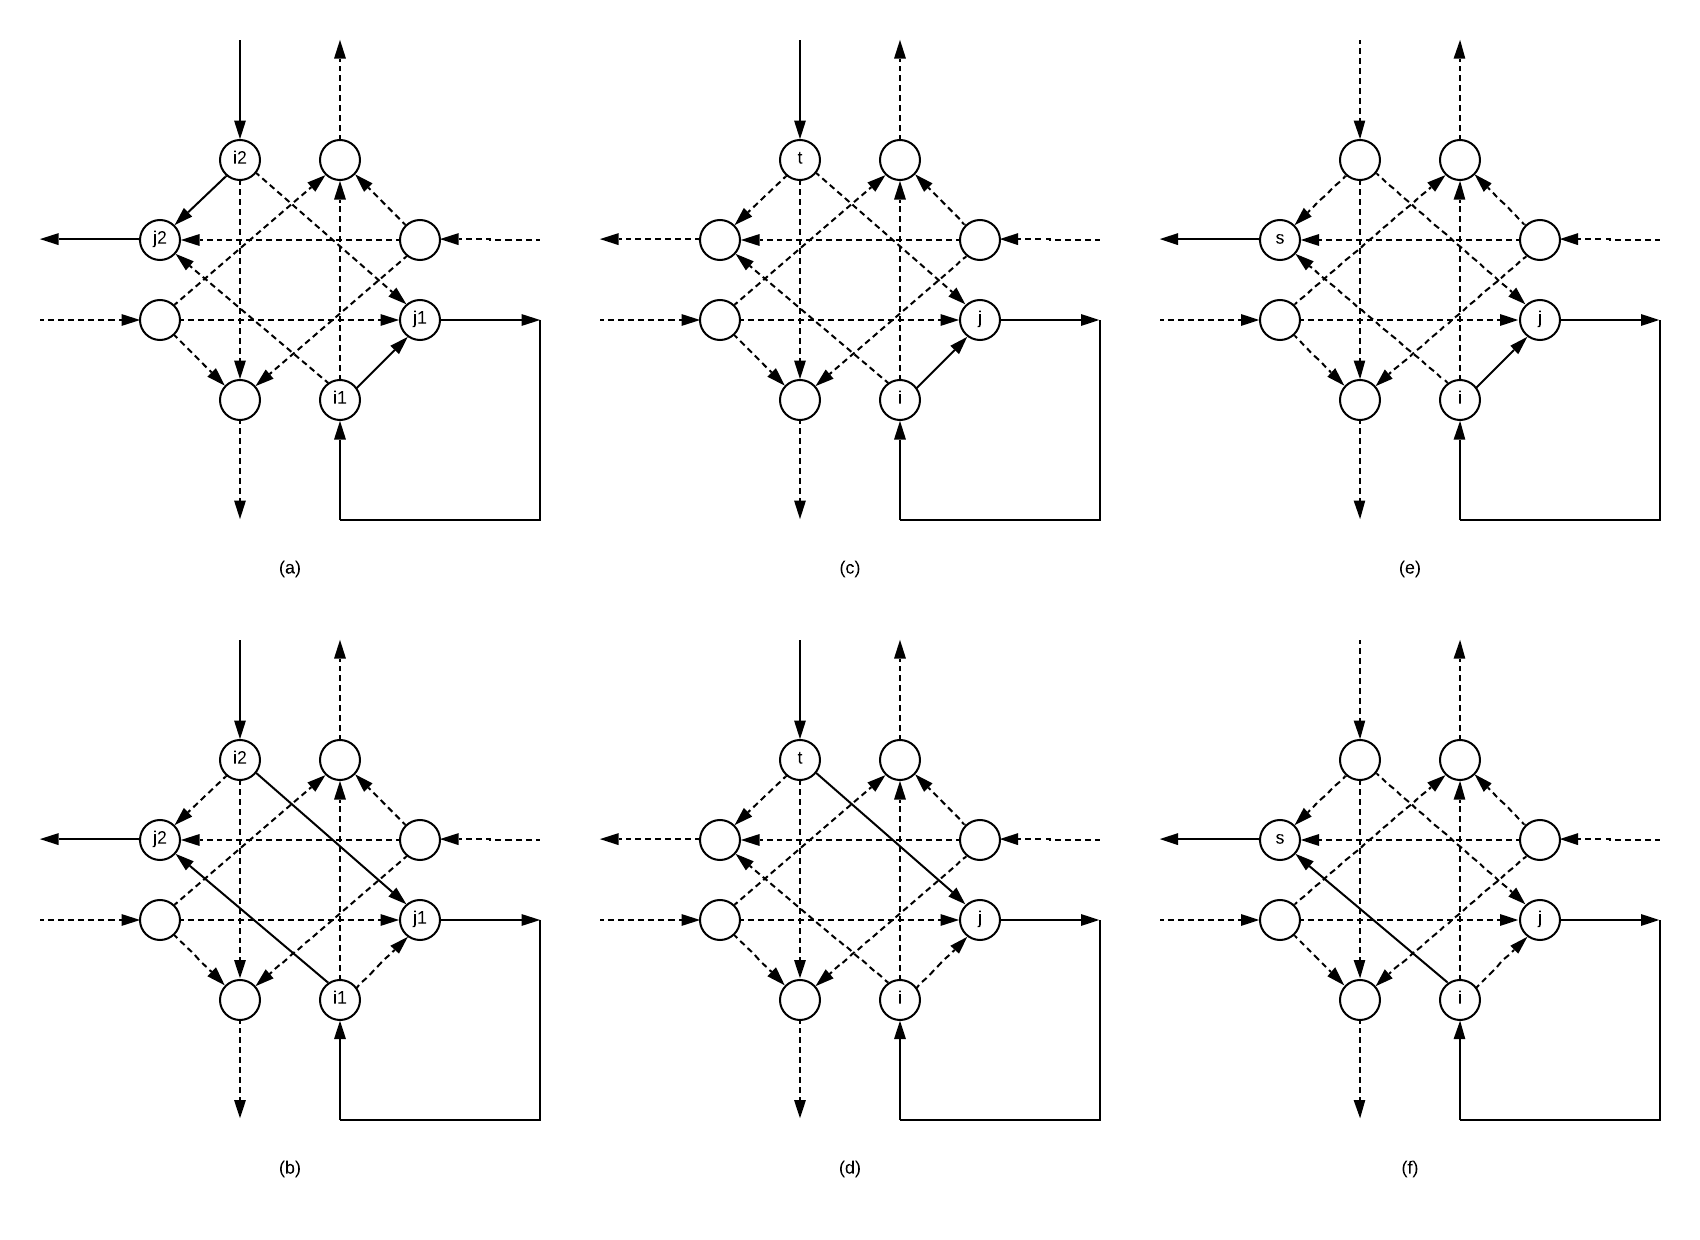
\includegraphics[width=13cm]{mezcla_subtours.png}}
\caption{Posibles configuraciones en el procedimiento de la mezcla de subtours. Si \textit{P} y \textit{S} tienen la configuración (a), (b) o (c), entonces la solución es modificada de acuerdo a lo especificado en (b), (d) o (f) respectivamente. [Fuente: \citet{Braier2017AnArgentina}]}
\label{fig:procedimiento_mezcla_subtours}
\end{figure}

Este procedimiento es aplicado para cada subtour en la solución hasta que todos sean mezclados al camino principal, dado que el costo de todos los arcos auxiliares que unen los nodos de las esquinas es el mismo, la ruta modificada permanece óptima, por lo que el algoritmo se detiene y devuelve la solución obtenida en este caso.

Dado que no siempre los subtours pueden ser mezclados con la técnica recién mencionada, el algoritmo principal descrito agrega una restricción estándar de eliminación de subtoures al modelo M, tal y como se especifica en el paso 6.

\subsection{Método de secuenciación}

% En este trabajo se realiza una búsqueda en profundidad para obtener la secuencia a seguir a partir del resultado del problema descrito en la sección anterior. El algoritmo toma como entrada el nodo inicial, nodo final y la cantidad de veces que se atraviesa por cada arco del grafo $G$. Se describe a continuación los pasos del algoritmo:

En este trabajo se realiza una búsqueda en profundidad para obtener la secuencia a seguir a partir del resultado del problema descrito en la sección anterior. El algoritmo recibe como parámetros de entrada el nodo inicial, nodo final, la cantidad de veces que se atraviesa por cada arco del grafo $G$ y un grafo dirigido $N$ construido teniendo en cuenta solo los arcos atravesados. Se describe a continuación los pasos del algoritmo:

\begin{enumerate}
\item Leer el grafo $N$ resultante del GDRPP abierto. 
\item Inicializar nodo actual al valor del nodo inicial.
\item Inicializar un vector vacío $seq$, en el que los nodos se almacenarán en el orden en que deben ser visitados.
\item Agregar a $seq$ el nodo actual.
\item Si el nodo actual es igual al nodo final y ya se atravesaron todos los arcos, entonces retornar $seq$ y parar.
\item Sino, tomar uno de los nodos sucesores del nodo actual en $N$, donde el arco formado por el nodo actual y el nodo sucesor aún no haya sido tenido en cuenta, asignar como nodo actual el nodo sucesor y volver al paso 4.
\end{enumerate}

\subsection{Ejemplo Numérico}
A continuación se describe un ejemplo simple de como la aplicación produce la secuencia del camino a seguir desde el resultado generado por la programación matemática.

El Paso 1 de la ``Fig.~\ref{fig:PasosSolucion}'' muestra los datos de salida que genera el modelo matemático (Algoritmo  de  solución, sección \ref{algoritmo-solucion}) a partir de un resultado factible. La salida contiene todos los segmentos que son utilizados como solución junto con el número de veces que se recorre cada uno de ellos, así como también despliega los nodos que resultaron elegidos como nodo inicial y nodo final del recorrido. Posteriormente, con estos datos se procede a crear un grafo dirigido con la cantidad total de arcos resultantes (Paso 2). El grafo generado pasa a formar parte de la entrada para obtener la secuencia del camino a seguir (Paso 3). Por último, el algoritmo de secuenciación se resuelve y genera como salida la secuencia de arcos del algoritmo de optimización.

\begin{figure*}[htbp]
\centerline{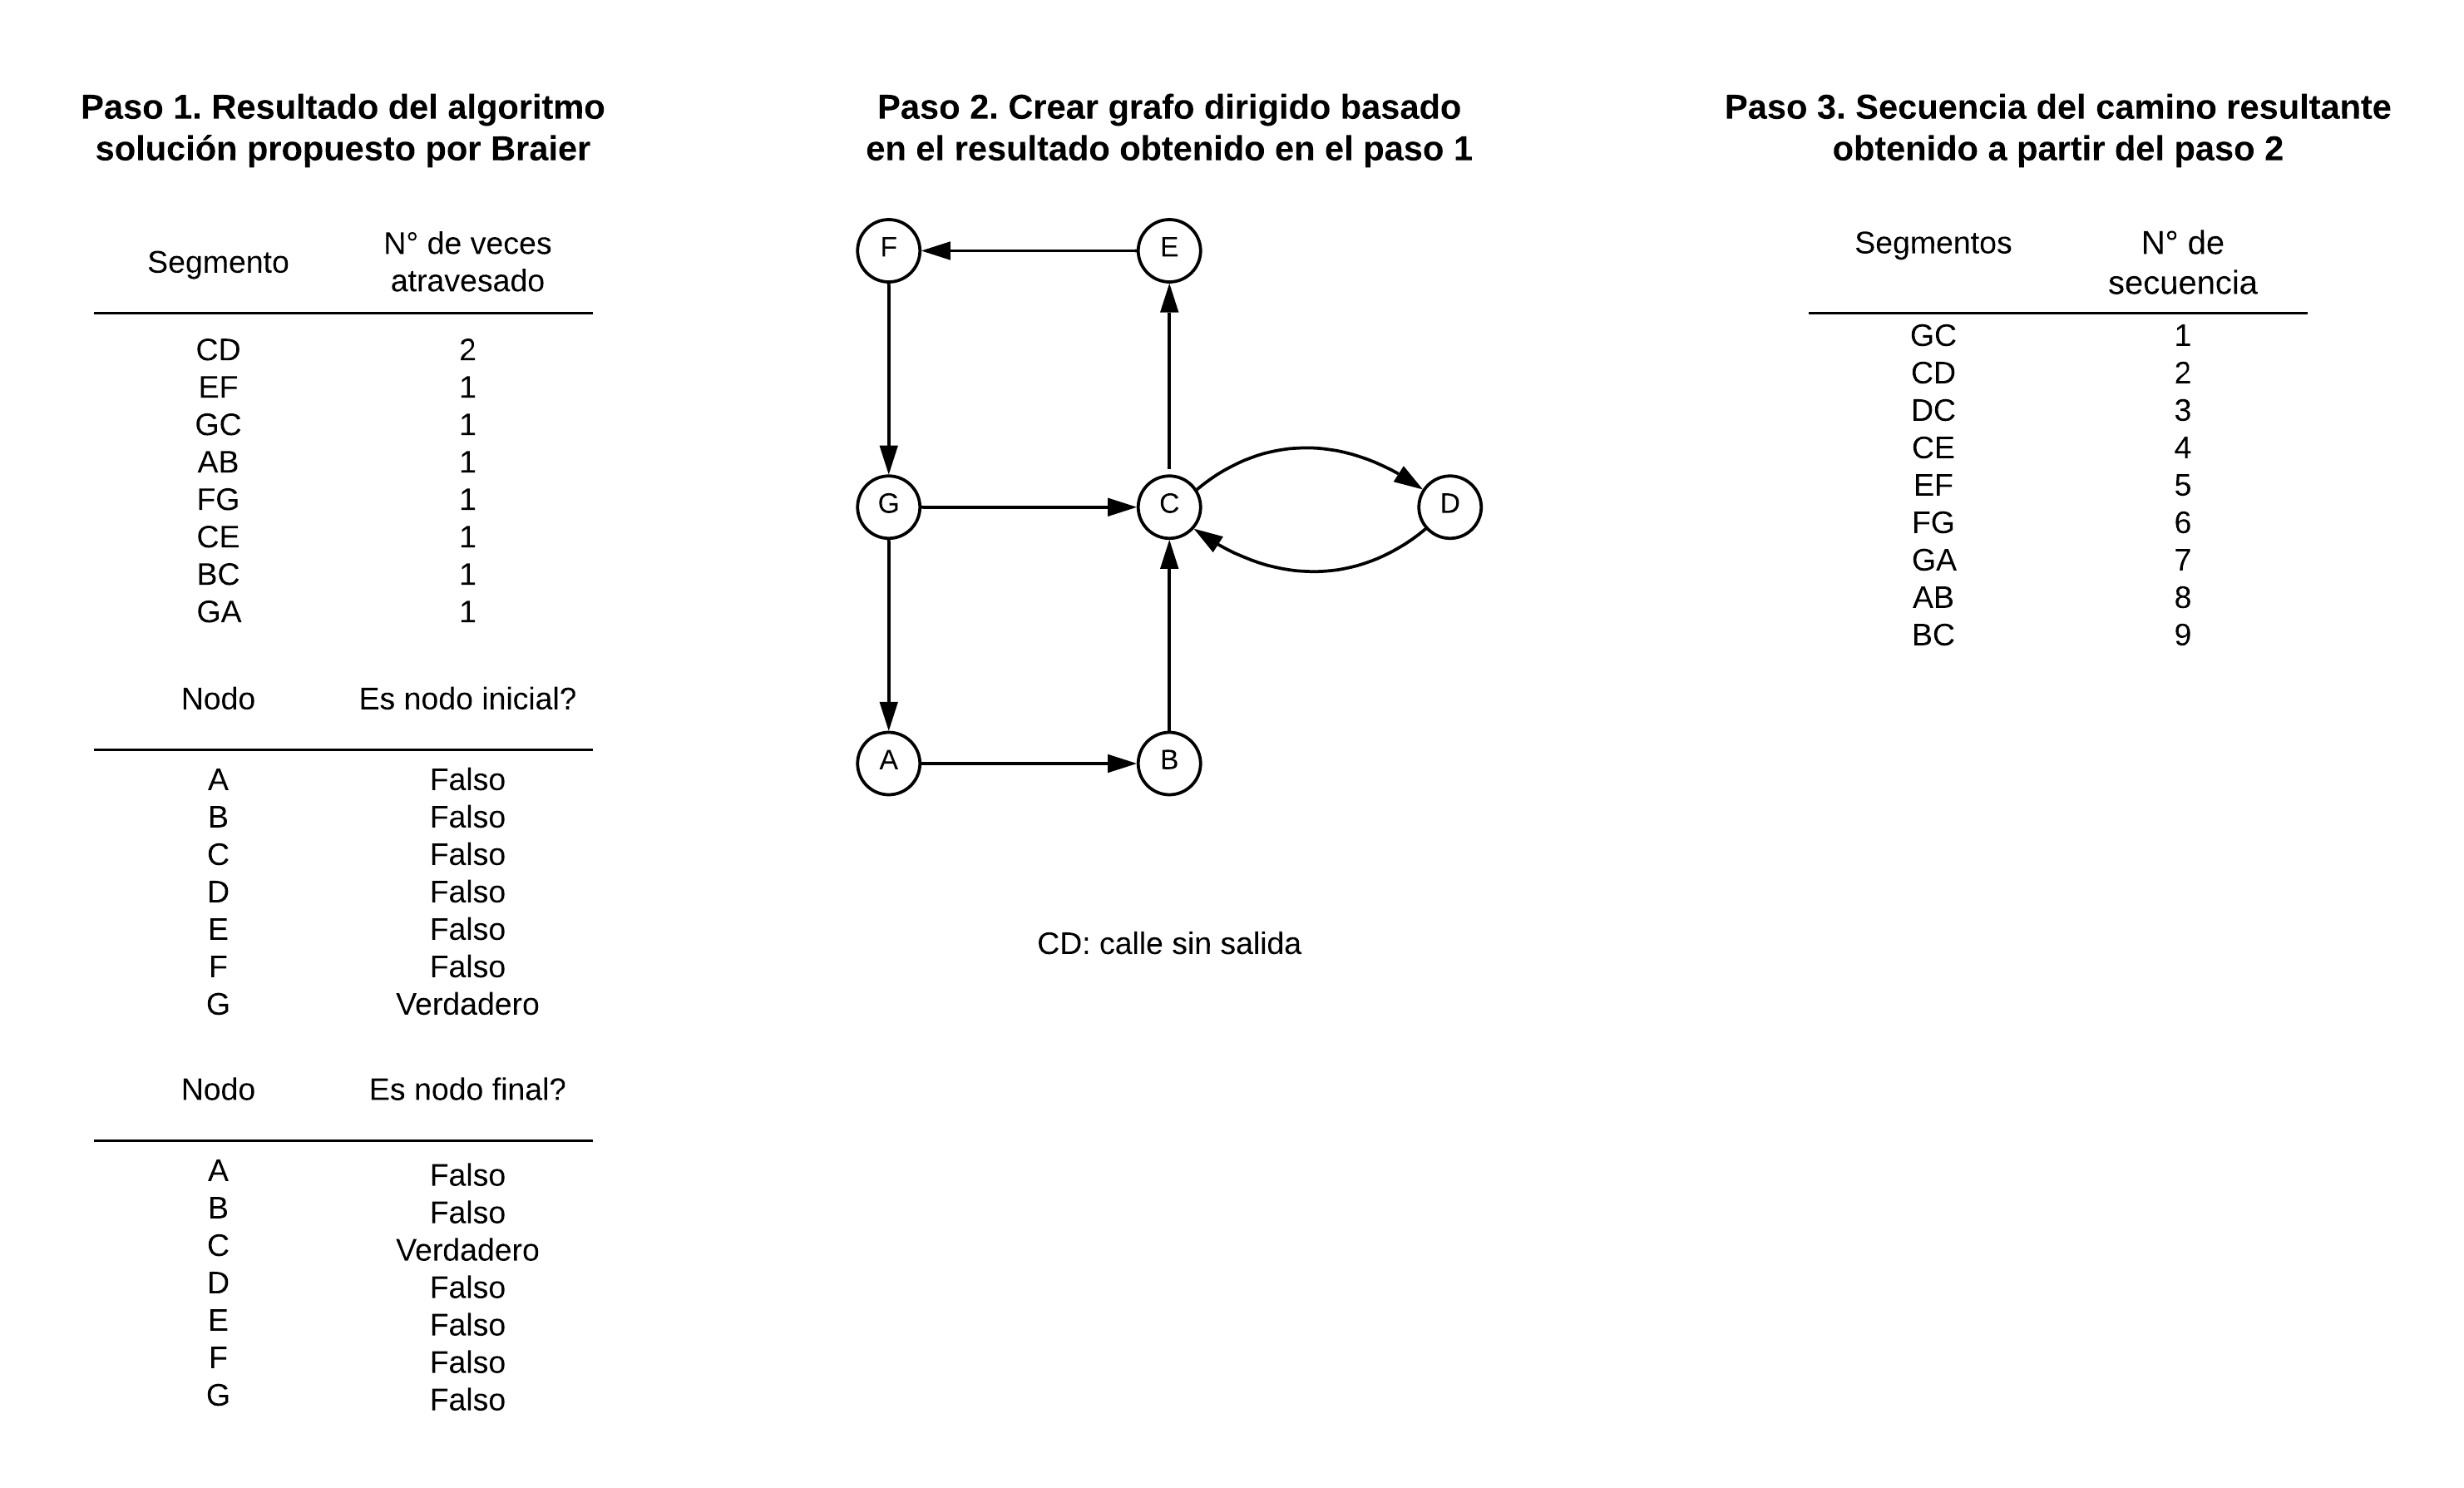
\includegraphics[width=\textwidth]{pasos_de_solucion.png}}
\caption{Pasos de solución para obtener la secuencia del camino del vehículo recolector en una zona.}
\label{fig:PasosSolucion}
\end{figure*}

\subsection{Solución propuesta}

En la actualidad, la DSU no cuenta con un \textit{Software} que apoye a la toma de decisiones en lo que respecta a la gestión de residuos sólidos urbanos, más específicamente en el área de recolección. Por lo tanto, se propone la implementación de una herramienta GIS que contribuya con la elección de mejores caminos a seguir por los vehículos recolectores, y de esta manera generar mayores beneficios en cuanto a tiempo y distancia, además de garantizar que el servicio sea brindado a todos los domicilios.
%además de contribuir con el cuidado del medio ambiente.

La implementación consta de los siguientes módulos:
\begin{enumerate}
    \item Seguridad: El sistema comprende un mecanismo de autenticación basada en tokens JWT (\textit{JSON Web Tokens}). Se restringe acceso a la aplicación y a los servicios web REST del servidor no autenticados.
    \item Administración: Comprende la gestión (listar, agregar, editar, eliminar) de usuarios, vehículos, turnos.
    \item GIS: Este módulo despliega el mapa con las diferentes capas (zona, calle, departamento, distrito) y permite el manejo de capas, la gestión de calles, generación de rutas, despliegue de resultado de ruta optimizada (Ver ``Fig.~\ref{fig:aplicacionRutas}'').
\end{enumerate}

La ``Fig.~\ref{fig:disenhoArquitectura}'' muestra el diseño de la arquitectura de \textit{software} alrededor de la aplicación solución \textit{TapeYty}. Este diseño se divide en dos partes que se explicarán en detalle a continuación.

\subsubsection{Cliente}

Desde una computadora portátil o un teléfono móvil el usuario puede acceder a la aplicación e ingresar con sus credenciales desde el navegador (\textit{browser}). Se ejecuta en el navegador el código Javascript generado a partir del código fuente construido con el marco (\textit{framework}) Angular (en su versión 7.0). Angular es un \textit{framework} ampliamente utilizado para el desarrollo de aplicaciones web con excelentes prestaciones en cuanto a rendimiento, escalabilidad, velocidad de respuesta y no menos importante una comunidad numerosa y activa. 

Una de las librerías incorporadas al proyecto cliente (\textit{frontend}) más relevantes para el trabajo es Mapbox GL JS, la cual ofrece funcionalidades relacionadas a mapas, teniendo como gran atractivo su buen desempeño durante el tiempo de renderizado de los mapas y datos geográficos.

\begin{figure}[tbp]
\centerline{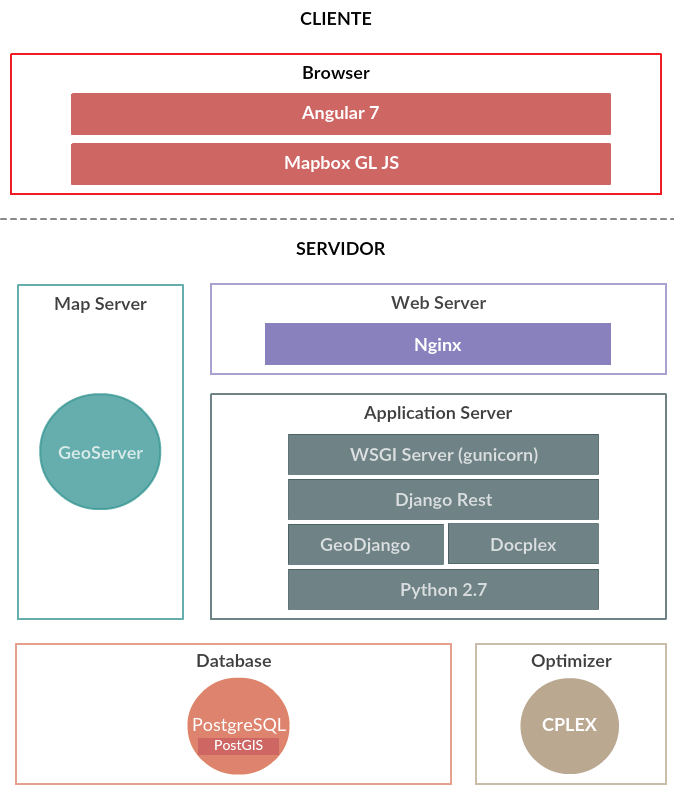
\includegraphics[width=8cm]{20190424_WebAppArchitectureDesign.png}}
\caption{Diseño de arquitectura de \textit{TapeYty}.}
\label{fig:disenhoArquitectura}
\end{figure}

\begin{figure*}[tbp]
\centerline{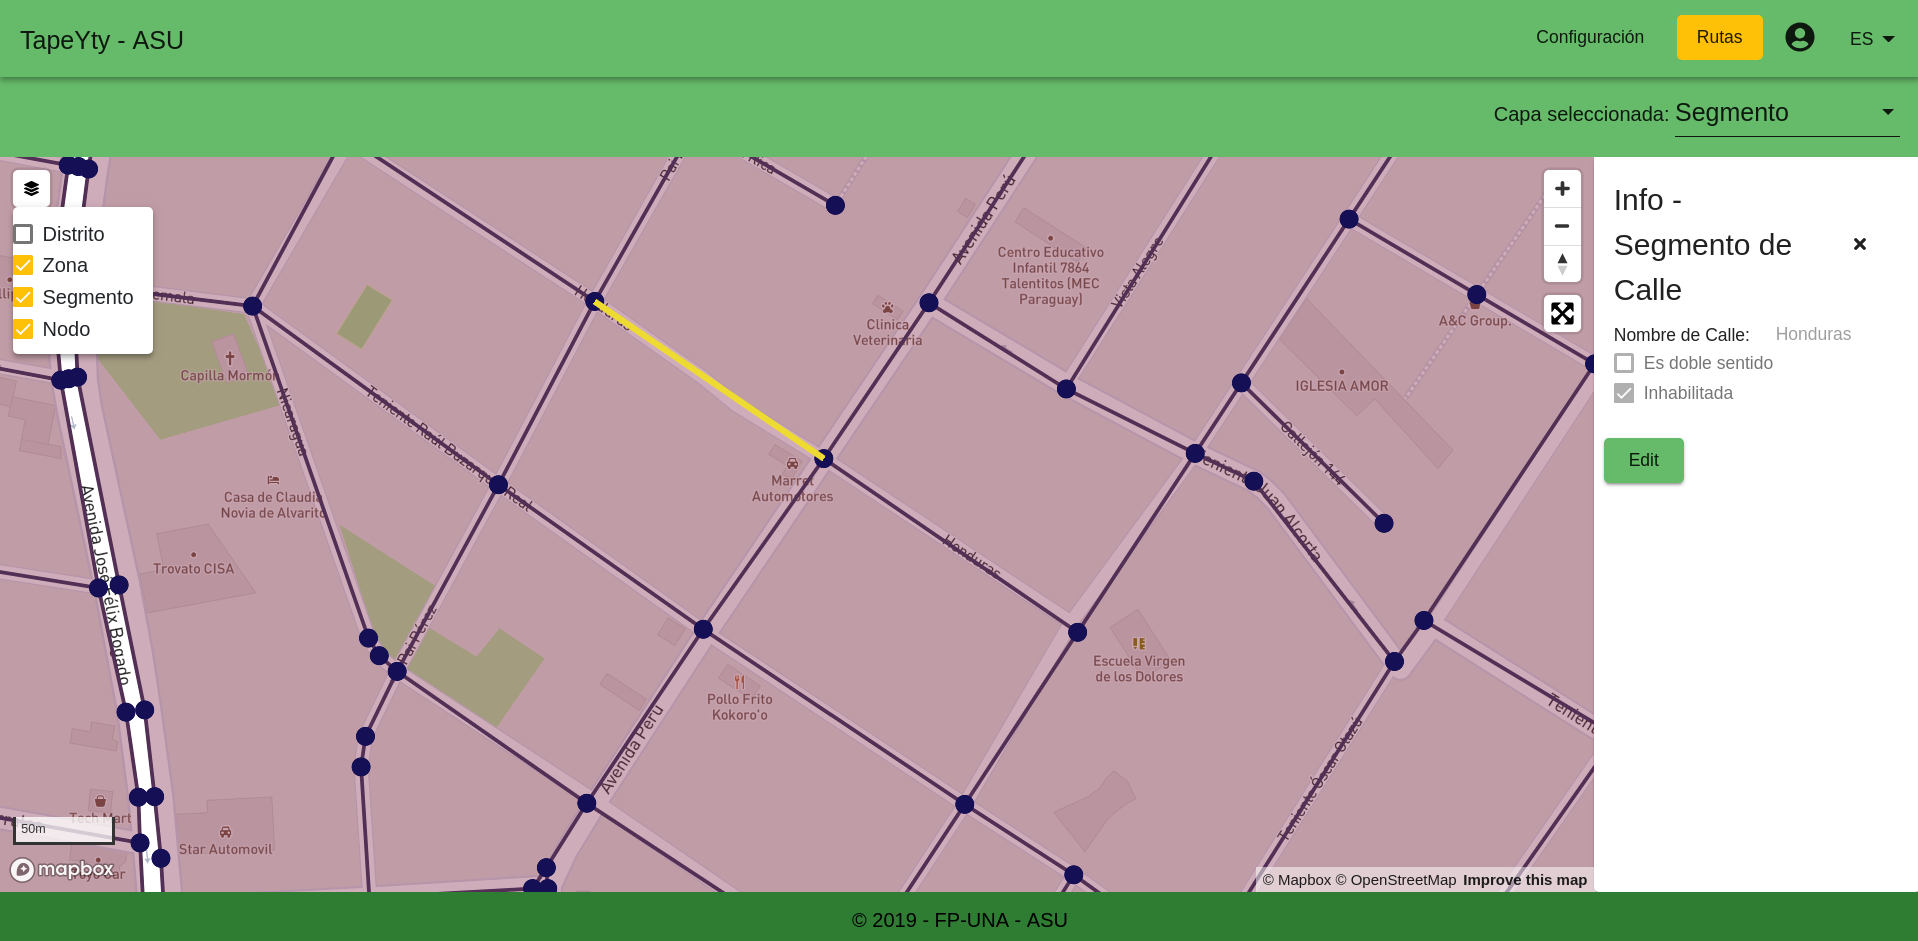
\includegraphics[width=\textwidth]{20190426_Aplicacion_Rutas.png}}
\caption{Edición de un segmento de calle en la aplicación \textit{TapeYty}.}
\label{fig:aplicacionRutas}
\end{figure*}

\subsubsection{Servidor}

El lado servidor presenta mayor complejidad ya que concentra varios componentes que además deben interactuar unos con otros.

Como parte de la solución, se utiliza el gestor de base de datos relacional PostgreSQL (versión 10.8) con su extensión PostGIS (version 2.4), donde están almacenadas las distintas informaciones obtenidas, geográficas o no, excepto los datos (\textit{shapes}) que provienen de la Dirección Nacional de Catastro de Paraguay.

El servidor de mapas GeoServer consiste en un servidor de código abierto escrito en Java que permite a los usuarios compartir y editar datos espaciales. En este servidor se almacenan los mapas bases de Departamentos y Distritos del Catastro Nacional. Además, se crea una conexión con la base de datos para poner a disposición las capas o mapas de calles y zonas, en modo lectura, donde el servidor ofrece servicios web de mapas como por ejemplo \textit{TMS} (\textit{Tile Map Service}), servicio que maneja estrategias de caché de cuadros de imágenes para mostrar los mapas con mayor velocidad dando un mejor rendimiento a la aplicación.

Para resolver el modelo matemático seleccionado se requiere de un \textit{software} especializado para ello. Se opta por la herramienta \textit{CPLEX Optimizer} de IBM en su versión académica, ya utilizado en trabajos previos \citep{Vecchi2016ACollection,Ramos2018TheApproaches,BabaeeTirkolaee2019DevelopingStudy}. El modelo matemático puede ser codificado en CPLEX con el lenguaje OPL ({\textit{Optimization Programming Language}}), provee además interfaces C, C++, Java y Python para su modelado. Sin embargo, estas interfaces no son usadas directamente para modelar sino a través de la librería Docplex detallada más adelante.

Para el desarrollo propio de una aplicación web una de las preocupaciones más importantes es la elección del lenguaje y el framework sobre los cuales estará construida. En este trabajo se opta por el lenguaje Python, conjuntamente con el framework GIS GeoDjango. En el área GIS, Python es uno de los lenguajes más utilizados a lo largo del tiempo, pudiéndose encontrar muchas funciones, librerías, \textit{software}, entre otros; escritos con este lenguaje. GeoDjango, basado en Django, tiene la virtud de ser robusto, provee un modelo de programación MVC (\textit{Model-View-Controller}) y facilita el desarrollo de aplicaciones Web.

La librería Docplex de Python resulta en una sencilla integración con nuestro \textit{framework}, también permite formular el modelo de forma clara y directa en comparación con las interfaces de CPLEX, resultando muy similar a la formulación con el lenguaje OPL.

Con Docplex y GeoDjango se implementa toda la lógica de negocio de la aplicación. Para poder acceder a esta lógica desde el cliente se requiere de una API (\textit{Application Programming Interface}). Para ello, se utiliza el protocolo de comunicación de intercambio de datos RESTful con la librería Django REST Framework y Django Rest Framework GIS. Se implementan los servicios para los módulos citados anteriormente como: agregar, eliminar y editar usuarios, editar propiedades alfanuméricas de calles, generar la ruta óptima de una zona, entre muchos otros; con estructuras de datos en formato JSON y geoJSON.

Con esto la aplicación está prácticamente lista, queda preparar el ambiente de producción para su implantación. Se instala uno de los servidores web más comunes actualmente, Nginx. El servidor web recibe una solicitud HTTP del cliente (el navegador), interpreta la solicitud y la envía a la puerta de enlace (\textit{gateway}). El \textit{gateway} Gunicorn es un servidor HTTP de Interfaz de Pasarela del Servidor Web de Python (WSGI, \textit{Web Server Gateway Interface}) que traduce la solicitud recibida del servidor web para que la aplicación pueda manejarlo. Y por el último tenemos la aplicación que a través de su API recibe la petición para luego procesarla y responderla.
